\documentclass[journal]{IEEEtran}

\usepackage{cite}
\usepackage{amsmath}
\usepackage{verbatim}%长篇注释宏包

\ifCLASSINFOpdf
\usepackage[pdftex]{graphicx}
\else
\fi

\hyphenation{op-tical net-works semi-conduc-tor}

\newcommand{\reffig}[1]{Fig. \ref{#1}}
\newcommand{\refsec}[1]{Section \ref{#1}}
\newcommand{\refeq}[1]{Eq. \ref{#1}}
\newcommand{\reftab}[1]{Table \ref{#1}}

\begin{document}
\title{A Noval Framework for Background Subtraction in Moving Camera}


% information of authors

\begin{comment}
\author{Chenqiu Zhao,
        Xiaohong Zhang and
		Sheng Huang, ~\IEEEmembership{Student Member,~IEEE}
		\thanks{Dan Yang is with School of Software Engineering,
		Chongqing University, Chongqing (401331), PR China.}
		\thanks{Chenqiu Zhao is with School of Software Engineering,
		Chongqing University, Chongqing (401331), PR China (e-mail: zhaochenqiu@gmail.com).}
		\thanks{Xiaohong Zhang is with Key Laboratory of Dependable
		Service Computing in Cyber Physical Society Ministry of
		Education, Chongqing (400044), P. R China, with School of
		Software Engineering, Chongqing University, Chongqing
		(401331), PR China, and with State Key laboratory of Coal
		Mine Disaster Dynamics and Control, Chongqing (400044), P. R
		China (e-mail: xhongz@cqu.edu.cn).}
		\thanks{Sheng Huang is with School of Software Engineering,
		Chongqing University, Chongqing (401331), PR China.}
		\thanks{Corresponding author: xhongz@cqu.edu.cn (X. H. Zhang),
		School of Software Engineering, Chongqing University, Huxi Town,
		Shapingba, Chongqing, P. R. China 410331.}}
\end{comment}
% The paper headers
%\markboth{Journal of \LaTeX\ Class Files,~Vol.~13, No.~9, September~2014}
%{Shell \MakeLowercase{\textit{et al.}}: Bare Demo of IEEEtran.cls for Journals}

% make the title area
\maketitle

% As a general rule, do not put math, special symbols or citations
% in the abstract or keywords.

%%%%%%%%%%%%%%%%%%%%%%%%%%%%%%%%%%%%%%%%%%%%%%%%%%%%%%%%%%%%%%%%%%%%%%%%
% Abstract															   %
%%%%%%%%%%%%%%%%%%%%%%%%%%%%%%%%%%%%%%%%%%%%%%%%%%%%%%%%%%%%%%%%%%%%%%%%
\begin{abstract}
\indent Background subtraction in moving camera is a challenging problem
in computer vision, since the position of pixels are varying during time
sequences and is hard to say what is background. In this paper, we assume
the main body of relative static part in scenes as the background, and 
proposed a novel framework named MDS(matching, detection and segmentation)
which utilize matching to counteract the displacement of camera and 
segmentation to improve the efficiency and robust of our framework. In MDS
we matching the image between two frames, and moving the background with
the frames. In this condition, the algorithms in static camera can work
in moving camera. And we utilized GMM to get the foreground. Moreover,
the matching point also showing the position of background. And 
we utilized the segmentation to mix the foreground and background.
Comprehensive evaluation demonstrates the superiority of framework 
against state of the art.
\begin{comment}
In this paper, we following the definition of background which
is the main body of relative static part in scenes, and proposed a novel
framework named MDS(matching, detection and segmentation) which utilize
matching to counteract the displacement of camera. In this condition, 

\indent The background subtraction is a challenging problem in computer
vision, since the all the position of pixels is change and is hard to said 
what is background. In this paper, we follows the means of background
which assume the relative static part and main part as background and 
proposed a novel framework named MDS(matching, detection and segmentation)
which utilize matching to counteract the displacement of camera moving.
In this condition, the algorithms in static camera like GMM can work in 
moving camera. Moreover, the matching point also show the background
information, in order to improve the robust and the efficiency of our
framework, we utilized segmentation to mix the foreground capture by
GMM and the background captured by matching point.
Comprehensive evaluation demonstrates the superiority of framework against state of the art.

\indent In background subtraction, the background is recognized as the static
part of scenes. But in video captured by moving camera, 
\indent Background subtraction is a crucial in computer vision. 
In preview work, many algorithms segment background by analysing the variation
of pixel's value, since the camera is assumed to be non-moving camera and
the position of pixel is not change. However, once the video is captured by
a free moving camera, all those algorithms is work hard. To solve this problem,
we proposed a novel framework named MSD(matching, segmentation and detection),
which 


utilize matching to counteract the displacement of camera, and the 
segmentation to improve the efficiency and robust of framework. In MSD, we 
assume the relatively static and main part is the background. In this assumption,
the matching algorithms also show the point of background. Then we utilized
segmentation to mix the foreground inforation by GMM, and the backgrond information
by matching point. Comprehensive evaluation demonstrates the superiority of 
framework against state of the art.

\indent The background is recognized as the static part of scenes in background
subtraction. In the preview work, people usually analysing the variation 
of pixel's value, since they assume the video is captured by non-moving camera.
However, once the camera produce some jitter or even dipacement, all those
algorthms will failed, which cause a challenge problem background subtraction

    Commonly, the background is recognized as the static part of scene.
So many algorithms segment background by analysing the variatin of pixel's
value, since all those work assumed the camera is a nonmoving camera. 
However, once the image sequences is captured by moving camerea, all those
algorithms will failed. To solve this problem, we present a novel framework
named MSD(matching, segmentation and detection) which assume the relative 
static part of scene as background. In MSD, the static part is capture by
mathcing algorithms. and the displacement of camera is reduce by it. In 
this condition, the moving camera is became static camera. And any algorithms
based on static camera can work well in moving camera. However, the error
is and we utilized segmentation algorithms to mix the foreground information 
and background information. Comprehensive evalution demonstrate our algorithms
get the state of the art in moving camera,and promissing result in  static 
camera.
\end{comment}
\end{abstract}

% Note that keywords are not normally used for peerreview papers.
\begin{IEEEkeywords}
Background Subtraction, motion, moving camera.
\end{IEEEkeywords}

\IEEEpeerreviewmaketitle

%%%%%%%%%%%%%%%%%%%%%%%%%%%%%%%%%%%%%%%%%%%%%%%%%%%%%%%%%%%%%%%%%%%%%%%%%
%																		%
% 1.Introdution														    %
%																		%
%%%%%%%%%%%%%%%%%%%%%%%%%%%%%%%%%%%%%%%%%%%%%%%%%%%%%%%%%%%%%%%%%%%%%%%%%
\section{Introduction}
\indent Background subtraction is a crucial problem in computer
vision, which has a wide range of applications including monitoring,
optical motion capturing and so on\cite{Han2012}. In the preview work, 
large numbers of algorithms assumed the camera is an Non-moving camera,
and segmented background by analysing the variation of pixels' value
\cite{Bouwmans2014}. However, in the free camera, the position of pixels
are varying during video sequences, it is hard to find a probabilistic
model for background subtraction.  To solve this problem, we proposed a 
novel framework named MSD(matching, segmentation and detection), which 
can let the algorithms in static camera can work in moving camera.\\
\indent Background is recognized as the static part of scenes. When
the video is captured by static camera, the value of pixels in background
is keep invariant, and a probabilistic model can be used for background
subtraction. However, in the video captured by moving camera, all the
position of pixels are change. In this condition, is hard to say what 
is background. To solve this problem, we follows the native means of
background and assume the main body of relatively static part in
scenes as background. Like \reffig{fig1} shown, the matching algorithms
can utilized to find the relatively static part. Then the GMM is used to 
detection the firegourd. Finally, segmntation algorithms is utilized to
mix the foregorund and background. \\
\begin{comment}
\indent Background is recognized as the static part of scenes. However
in the video captured by moving camera, it is hard to say what is 
background, sinceall the position of pixels is change. In this condition
, we follows the native means of background which is the main body of 
relative static part in scenes. Like the figure shown. The mathcing algorithms
can utilized to find those part. Then the matrix can be captured by those
part. Then, the segmentation can be utilized to mix the foreground and
background. \\
\end{comment}
% /%%%%%%%%%%%%%%%%%%%%%%%%%%%%%%%%%%%%%%%%%%%%%%%%%% figure:fig1
\label{fig1}
\begin{figure}[!t]	% FIGURE: figure/fig1 
\centering
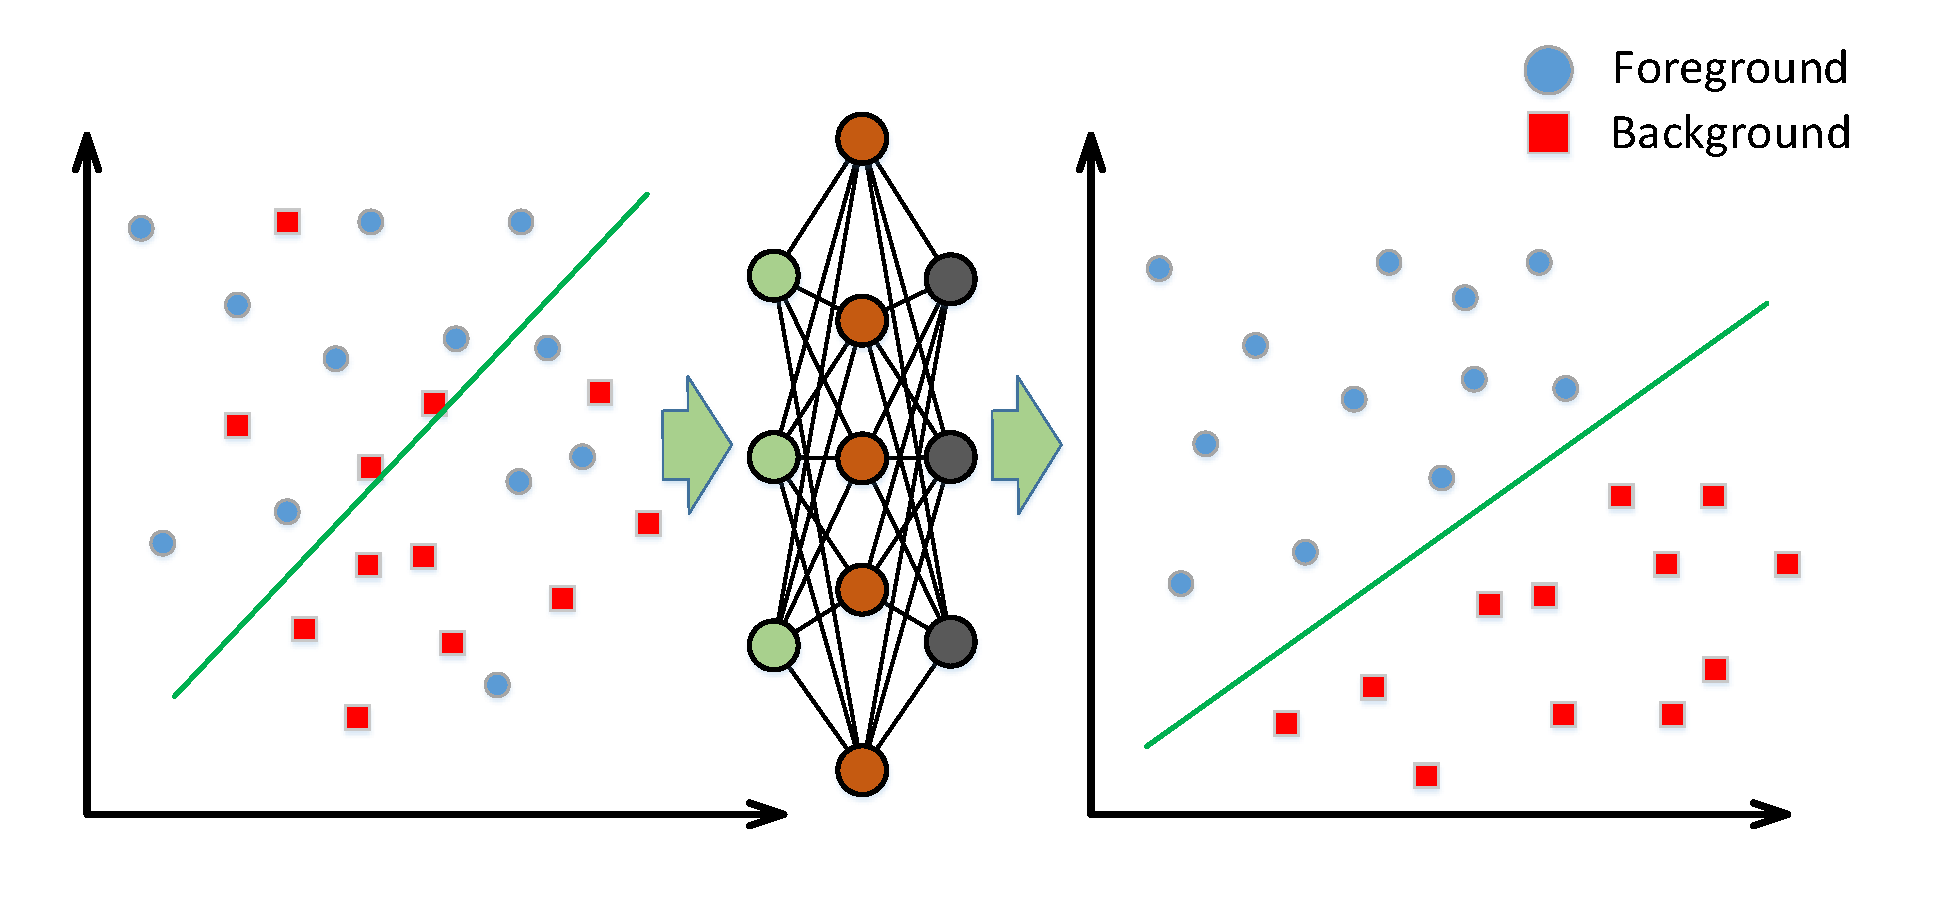
\includegraphics[width=3.5in]{figure/fig1}
\DeclareGraphicsExtensions.
\vspace{-10pt}
\caption{The illustration of complex scenes are recognized as the
mixture of R1, R2, R3, R4 and R5 which characterized by green color,
gray, texture, red color and blue color as dominant features,
respectively. Different dominant features are utilized for modelling
the background in each zone.}
\label{fig1}		% LABEL: fig1
\end{figure}
% %%%%%%%%%%%%%%%%%%%%%%%%%%%%%%%%%%%%%%%%%%%%%%%%%%/ figure:fig1
\indent In MDS framework, matching algorithms is used to matching the displacement
of two frames. We set a plot in four dimenstrate. In this condition, the camera
is become static camera. And all the algorithms based on static camera can
work well in moving camera. However, the matching algorithms can get no error.
And for solve this problem, we need to improve the robust. We used segmentation
the image into several segments And count the foreground and background for
the finally result. In fact, so we scale the segment in different scale.for 
the finally background. We utlized the GMM into our framework, and apply our 
work to some standard change detection dataset. The comparion of out algorithms
with other state of art in different videos shown that proposed approach state
of art approaches.
\begin{comment}
In this condition, the matching can used 
to find those part, and captured the matrix. For those, the displacement of
camera can be counteract, and the 

\indent In moving objects detection, the background is recognized 
Background subtraction in moving camera is a challenging 
Background subtraction has a wide range of applications, 
\indent Background subtraction has a wide range of applications, including video
monitoring[], optical motion capturing[] and multimedia applications[].
In preview work, so many algorithms labeled a pixel as background when 
the variation of it is keep invariant, since they assumed the camera is
a non-moving camera. However, in the real work, the moving camera is 
everywhere and has many challenging problem. This paper assume the relative
static part as background which found the relative staic part of scene 
instead of analysing the value of pixle in time sequences.
\indent The background is recognized as the staic part of scene. However
in the video captued by moving camera, all the position of pixel is
changing, which caused large different to segment background by analysing 
pixel's value. 
\indent In this work, we assume the backgroud in moving camera is the
relatively static and main part scene. We used SIFT feature point and 
ransac to mathcing image, to reduce the camera moving. Then the algorithms
in static camera can work well in the moving camera. and  we used gmm to
get the foreground information. In the same time, the ransac algorithms
also show the background part of scene. And we used superpixel to solve
this problem.
here is introduction.\cite{Stauffer1999}
\end{comment}
%%%%%%%%%%%%%%%%%%%%%%%%%%%%%%%%%%%%%%%%%%%%%%%%%%%%%%%%%%%%%%%%%%%%%%%%%
%																		%
% 2.Related work														%
%																		%
%%%%%%%%%%%%%%%%%%%%%%%%%%%%%%%%%%%%%%%%%%%%%%%%%%%%%%%%%%%%%%%%%%%%%%%%%
\section{Related work}
\indent Recently, many impressive work were proposed for background subtraction
in moving camera. In this paper, we divided those algorithms in two
categories. The first categories try to find the new stable features to
segment background. The second categories is focus on how to reduce
the displacement of camera moving, and our work is belong to the second
categories.
\subsection{Algorithms based on new stable features}
\subsection{Algorithms focus on counteract camera moving}
%%%%%%%%%%%%%%%%%%%%%%%%%%%%%%%%%%%%%%%%%%%%%%%%%%%%%%%%%%%%%%%%%%%%%%%%%
%																		%
% 3.Feature extraction													%
%																		%
%%%%%%%%%%%%%%%%%%%%%%%%%%%%%%%%%%%%%%%%%%%%%%%%%%%%%%%%%%%%%%%%%%%%%%%%%
\section{The MSD framework}
\indent In this section, we explaining the processing of MSD. In, we introduction
how to let the algorithms in static can work in moving camera. In , how
to mix the foreground and background.
\subsection{The moving of camera}
\indent The processing of counteract moving of camera is shown like Fig2.
We set a plot in time sequences to like the background moving with camera
moving.
\indent In MSD, we are try counteract the moving of camera. Let's donate
the frames of video is ${f_1,f_2,...f_n}$ .There are two matching, the first
matching is used two frames $f_i$ and $f_{i+1}$The background, the matrix
 is $H$
, then we rotate the image intothen we get the 
\begin{displaymath}
    f'(x,y) = f(x,y)H.
\end{displaymath}
\indent The second matching is for best background and the frames to get
the background information.
\subsection{Mixing of foreground and background}
herer is feature extraction.
%%%%%%%%%%%%%%%%%%%%%%%%%%%%%%%%%%%%%%%%%%%%%%%%%%%%%%%%%%%%%%%%%%%%%%%%%
%																		%
% 4. Modeling the background with multi-feature							%
%																		%
%%%%%%%%%%%%%%%%%%%%%%%%%%%%%%%%%%%%%%%%%%%%%%%%%%%%%%%%%%%%%%%%%%%%%%%%%

%%%%%%%%%%%%%%%%%%%%%%%%%%%%%%%%%%%%%%%%%%%%%%%%%%%%%%%%%%%%%%%%%%%%%%%%%
%																		%
% 5.Experiments															%
%																		%
%%%%%%%%%%%%%%%%%%%%%%%%%%%%%%%%%%%%%%%%%%%%%%%%%%%%%%%%%%%%%%%%%%%%%%%%%
\section{Experiments}
In this section, we compare our framework with XXX state-of-art algorithms
in different dataset.
%%%%%%%%%%%%%%%%%%%%%%%%%%%%%%%%%%%%%%%%%%%%%%%%%%%%%%%%%%%%%%%%%%%%%%%%%
%																		%
% 6.Conclusion															%
%																		%
%%%%%%%%%%%%%%%%%%%%%%%%%%%%%%%%%%%%%%%%%%%%%%%%%%%%%%%%%%%%%%%%%%%%%%%%%
\section{Conclusion}
here is conclusion
%%%%%%%%%%%%%%%%%%%%%%%%%%%%%%%%%%%%%%%%%%%%%%%%%%%%%%%%%%%%%%%%%%%%%%%%%
%																		%
% 7.Acknowledgement														%
%																		%
%%%%%%%%%%%%%%%%%%%%%%%%%%%%%%%%%%%%%%%%%%%%%%%%%%%%%%%%%%%%%%%%%%%%%%%%%

\begin{comment}

\section*{Acknowledgement}
\noindent The work described in this paper was partially supported by the National
Natural Science Key Foundation (Grant no. 91118005), the National
Natural Science Foundation of China (Grant no. 61173131), the Natural
Science Foundation of Chongqing (Grant no. CSTS2010BB2061), the
Fundamental Research Funds for the Central Universities (Grant Nos.
CDJZR12098801 and CDJZR11095501) and the Chongqing Graduate Student
Research Innovation Project (Grant no. CYB14034).	\\

\end{comment}
\ifCLASSOPTIONcaptionsoff
  \newpage
\fi

  
 %\bibliographystyle{plain}
 %\bibliography{ref}


\bibliographystyle{IEEEtran}  
\bibliography{ref_abb}  

\begin{comment}
\begin{IEEEbiographynophoto}{Dan Yang}
received the B.Eng. degree in automation,
the M.S. degree in applied mathematics, the
Ph.D. degree in machinery manufacturing and
automation from Chongqing University, Chongqing.
From 1997 to 1999, he held a postdoctoral position
with the University of Electro-Communications,
Tokyo, Japan. He is the Vice President of
Chongqing University, and a  Professor with the
School of Software Engin
eering. He has authored
over 100 scientific papers and some of them
are published in some authoritative journals and conferences,  such  as  the  IEEE  TRANSACTIONS  ON PATTERN ANALYSIS AND MACHINE INTELLIGENCE, CVPR, and BMVC. His research interests
include computer vision, image proce
ssing, pattern recognition, software
engineering, and scientific computing.
\end{IEEEbiographynophoto}


\begin{IEEEbiographynophoto}{Chenqiu Zhao}
\end{IEEEbiographynophoto}


\begin{IEEEbiographynophoto}{Xiaohong Zhang}
\end{IEEEbiographynophoto}

\begin{IEEEbiographynophoto}{Sheng Huang}
(S' 14) received the B.Eng. degree in software engineering and the Ph.D. degree in computer science from Chongqing University,
Chongqing, in 2010 and 2015, respectively. From
2012 to 2014, he was a Visiting Student with the
Department of Computer Science, Rutgers Univer-
sity, Piscataway, NJ, USA. He has authored several
scientific papers in venues, such as CVPR, BMVC,
ICME, ISBI, and ICIP. His research interests include
pattern recognition, computer vision, machine
learning, and biometrics.
\end{IEEEbiographynophoto}
\end{comment}

%\begin{IEEEbiography}{Dan Yang}
%Biography text here.
%\end{IEEEbiography}

\end{document}
